
%%%%%%%%%%%%%%%%%%%%%%%%%%%%
%\subsection{Validation of Calibration Hardware Systems}
%\label{sec:sp-calib-val}
%\fixme{Validation section. JM: Done. SG/KM: please check.}

All the designs presented above have aspects that warrant a validation in a situation as close as possible to the final one to be deployed in DUNE FD. Tests in member institute laboratories needed to converge on a baseline design are described in the earlier sections. Here, we describe the validation of a complete baseline design.

Even if there are laser calibration systems in operation in other \dword{lar} TPC experiments (e.g. MicroBooNE, future SBND runs), the stringent requirements of such a system in terms of mechanical and optical precision, long-term reliability, track length, impact on \efield in case of an alternative design, and DAQ interface all lead to corresponding goals of a test installation and operation in dword{pdsp}, that could be accomplished in the post-LS2 run. As can be seen in Fig.~\ref{fig:pDmap}, there are currently ports of the same size as DUNE-FD that could possibly be used for these tests. If a pair of ports are used, then one could even have crossing tracks within a single drift volume. 

The goal of this would be to test all aspects of the system design, installation, alignment, operation, interfaces with DAQ, analysis, etc. In \dword{pdsp}, due to its location at surface, it should be possible to obtain a measurement of the \efield map with cosmics, and compare it with the one from the laser system, in order to improve the analysis methods or identify weak points in the design. An important design parameter is the length of a laser track. Our design assumes that 20 m is possible, but microBoone has demonstrated up to 10 m, but it could be larger, and also depend on laser intensity. Measurements are limited by the size of the detector, but a way to gain information on possible higher lengths would be to make a scan with low laser intensities, such that and end of the track would visible and register how the maximum obtained track length scales with intensity. An extrapolation to the DUNE \dword{fd} laser intensity would tell us what the maximum length would be there. Such a measurement could also be done at 
MicroBOONE or SBND.

\begin{figure}[tbp]
\centering
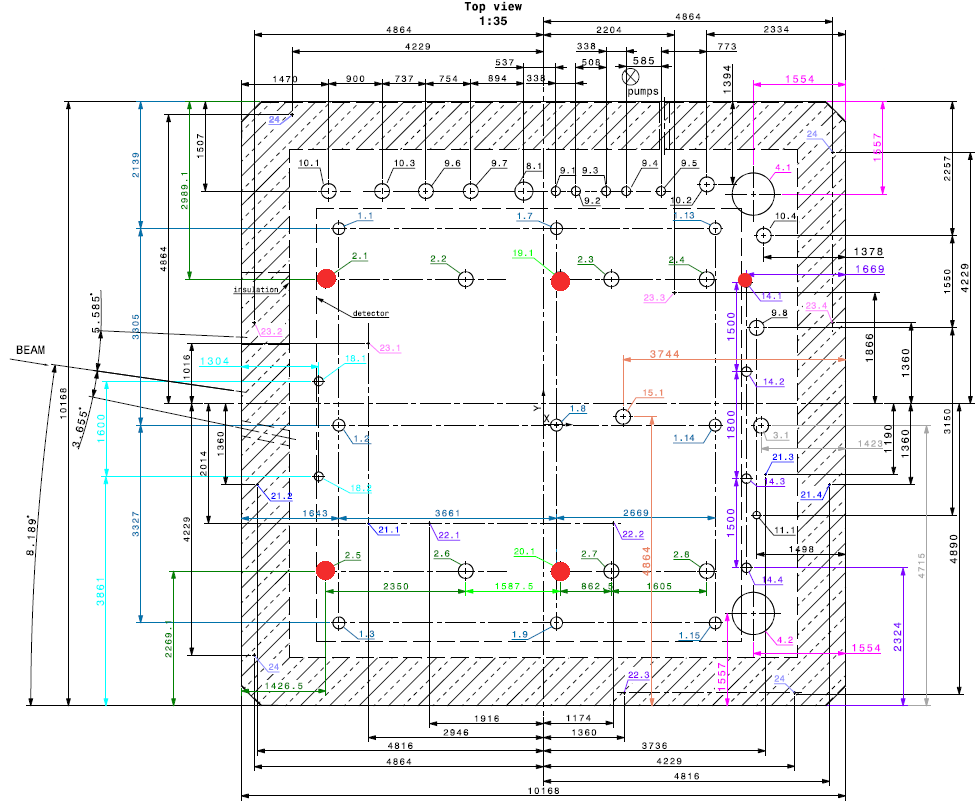
\includegraphics[height=4.0in]{graphics/protoDUNESP_topView_marked.png}
\caption{Top view of the dword{pdsp}
cryostat showing various penetrations. Ports marked in red are present free and they could be used for tests of the calibration systems. The four largest ones have the same diameter (250 mm) of the calibration ports of DUNE \dword{fd}, and are located over the TPC. The two larger ports at the right-hand side corners of the cryostat are the human access ports (or manholes).}
\label{fig:pDmap}
\end{figure}

The pulsed neutron source is a new idea that has never been used in other experiments, so a \dword{pdsp} test is especially important. The corner human access ports similar to DUNE FD could be used for this deployment.
%The post-beam run being proposed for ProtoDUNE-SP offers the opportunity to test the full system (DD Generator, Moderator, Transport Model, Data Analysis) in a definitive way before investing in the full PNS calibration for DUNE. The PNS group proposes to make such a run as soon as resources can be identified (independent of the other measurements above), starting with a commitment of engineering resources at CERN required to complete the necessary radiation safety shield design, and the mechanical design necessary to support the DD Generator and Moderator. The system used for ProtoDUNE-SP could also be used for ProtoDUNE-DP, and later installed in the DUNE detector. 

With respect to the radioactive source system, the cosmic induced background rate is too high at surface to detect the response to the DUNE gamma source; a higher intensity source can be considered to be deployed to test the detector response and analysis method. However, tests of functionality,  reliability, and safety of the mechanical deployment system are needed to demonstrate the source can be deployed and retrieved with no issues.

In addition to dedicated hardware validation runs at \dword{pdsp} running, other liquid argon experiments are providing ample opportunities for development and validation of calibration tools and techniques, especially those that are relevant for the hardware being deployed. For example, the MicroBooNE experiment is currently leading the development of analysis methods using laser data to extract an \efield map. Additionally, energy calibration techniques and related software tools are being developed at various experiments (MicroBooNE, ICARUS, LArIAT, ProtoDUNE) that involve estimating and propagating uncertainties like \efield distortions, recombination etc. into physics signals. Other calibration related developments include DAQ and calibration database design, all of which are being honed at SBN and ProtoDUNE.
 
%%%%%%%%%%%%%%%%%%%%%%%%%%%%
%\subsubsection{Validation in Other Experiments}
%\label{sec:sp-calib-val-other}

%\cleardoublepage